\documentclass[tikz,border=5pt]{standalone}
\usepackage{tikz}
\usetikzlibrary{arrows,arrows.meta,automata,positioning,calc}

\begin{document}
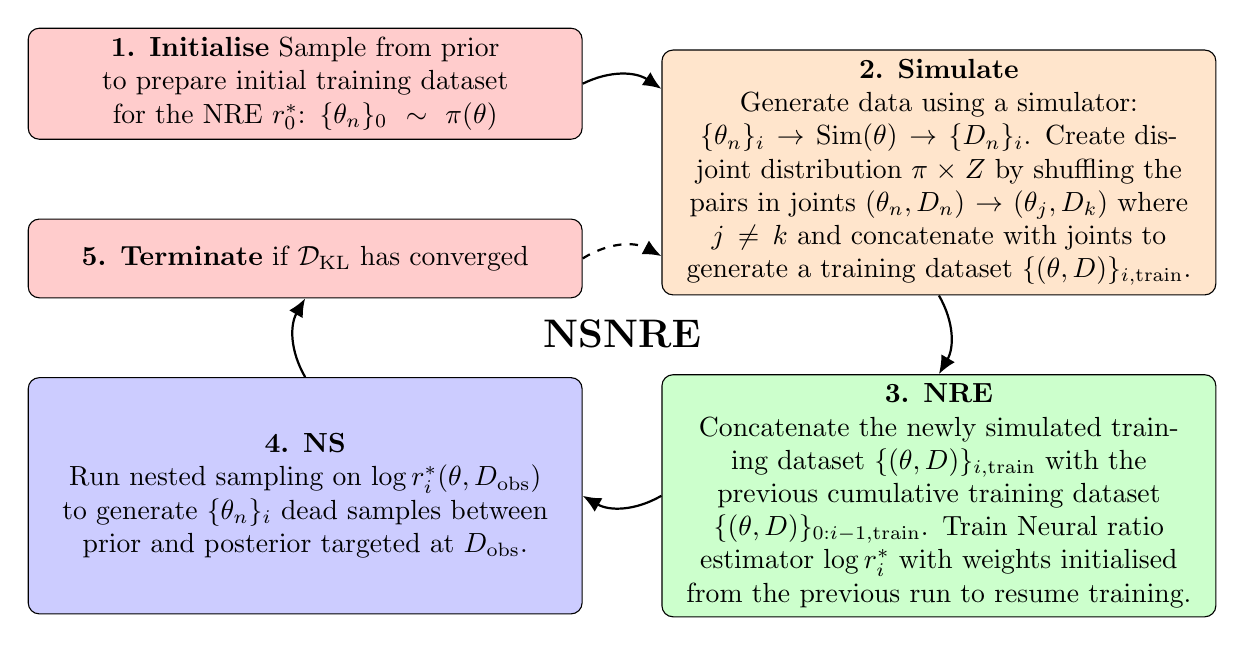
\begin{tikzpicture}[
        node distance=1cm,
        >=stealth, auto,
        every state/.style={
            rectangle, rounded corners, minimum width=2em,
            text width=6.8cm, align=center
        }
    ]
      \node[state, fill=blue!20, minimum height=3cm] (q14) {
        \textbf{4. NS}\\
        Run nested sampling on $\log r^*_{i}(\theta, D_\mathrm{obs})$ \\
        to generate $\{\theta_n\}_i$ dead samples between prior and posterior targeted at $D_\mathrm{obs}$.

    };
    \node[state, fill=red!20, minimum height=1cm] (q121) [above=of q14] {
        \textbf{5. Terminate} if $\mathcal{D}_\mathrm{KL}$ has converged
    };
    \node[state, fill=red!20, minimum height=1cm] (q12) [above=of q121] {
        \textbf{1. Initialise} Sample from prior to prepare initial training dataset for the NRE $r^*_0$: $\{\theta_n\}_0 \sim\pi(\theta)$ \\
    };
    \node[state, fill=green!20, minimum height=3cm] (q34) [right=of q14] {
        \textbf{3. NRE}\\
        Concatenate the newly simulated training dataset $\{ (\theta,D)\}_{i, \mathrm{train}}$ with the previous cumulative training dataset $\{ (\theta,D)\}_{0:i-1, \mathrm{train}}$.
        Train Neural ratio estimator $\log r^*_i$
        with weights initialised from the previous run to resume training. };
    \node[state, fill=orange!20, minimum height=3cm] (q23) [above=of q34] {
        \textbf{2. Simulate}\\
        Generate data using a simulator: $\{\theta_n\}_i \to \mathrm{Sim(\theta)} \to  \{D_n\}_i$. Create disjoint distribution $\pi \times Z$ by shuffling the pairs in joints $(\theta_n, D_n) \to (\theta_j, D_k)$ where $j \neq k$ and concatenate with joints to generate a training dataset $\{ (\theta,D)\}_{i, \mathrm{train}}$.
    };
    \begin{scope}[bend left]%
        \path[thick,-{Latex[width=2mm]}]   (q14.north) edge node {} (q121.south)
        (q121.east) edge[dashed] node {}($(q23.south west)!0.16!(q23.north west)$)
        (q23.south) edge node {} (q34.north)
        (q34.west) edge node {} (q14.east)
        (q12.east) edge node {}($(q23.south west)!0.84!(q23.north west)$) ;
    \end{scope}

    \node[align=center] (e) at (barycentric cs:q121=0.5,q12=0.5,q23=1,q34=1,q14=1) {\Large\textbf{NSNRE}};
\end{tikzpicture}
\end{document}
